\chapter{Боулинг}

В този проект ще създадете една любима игра на детацата - боулинг. Играчът ще трябва да изстреля топка от долната част на екрана, която ще достигне до кеглите, които се намират в горната част. Целта е играчът да събори всички кегли.

\begin{figure}[H]
  \centering
  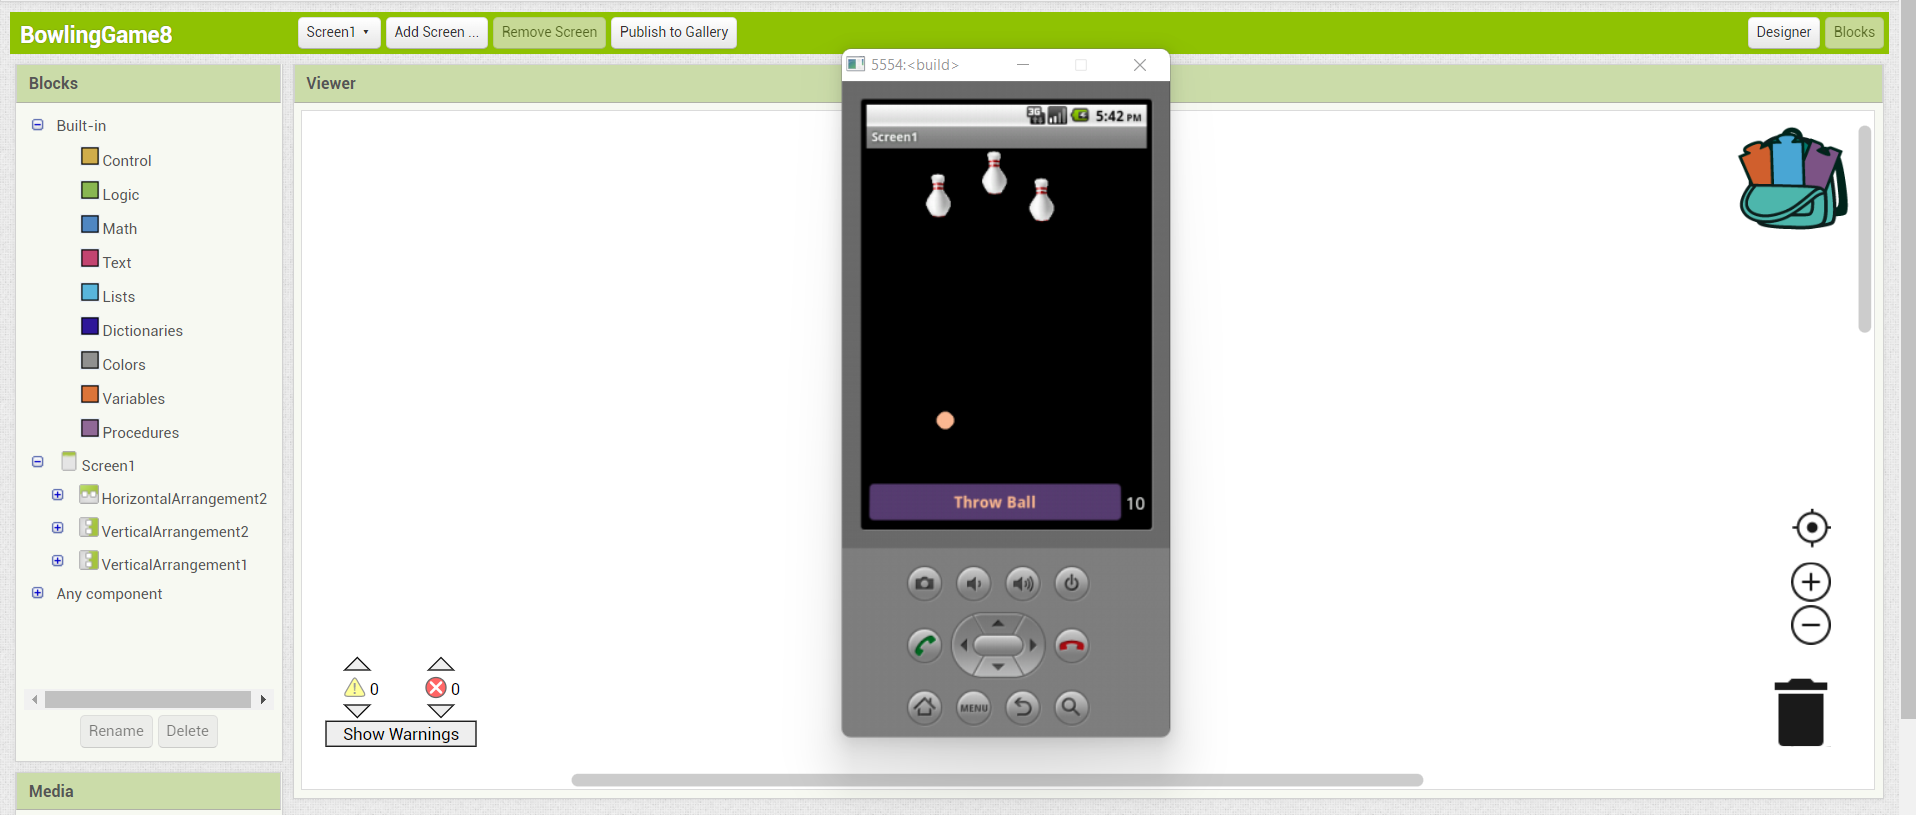
\includegraphics[width=1.0\linewidth,height=0.5\linewidth]{fig130001.png}
  \caption{Боулинг}
\label{fig130001}
\end{figure}

\section{Създаване на дизайна}

В първата стъпка ще създадете началният екран на играта. Върху него ще има един бутон, който ще бъде начало на играта. От групата с елементите Layout трябва да бъде добавен елемента VerticalArrangement. Размерите на елемента трябва да бъдат такива, каквито са размерите на екрана. За това свойствата за височина и ширина трябва да се сменят.

\begin{figure}[H]
  \centering
  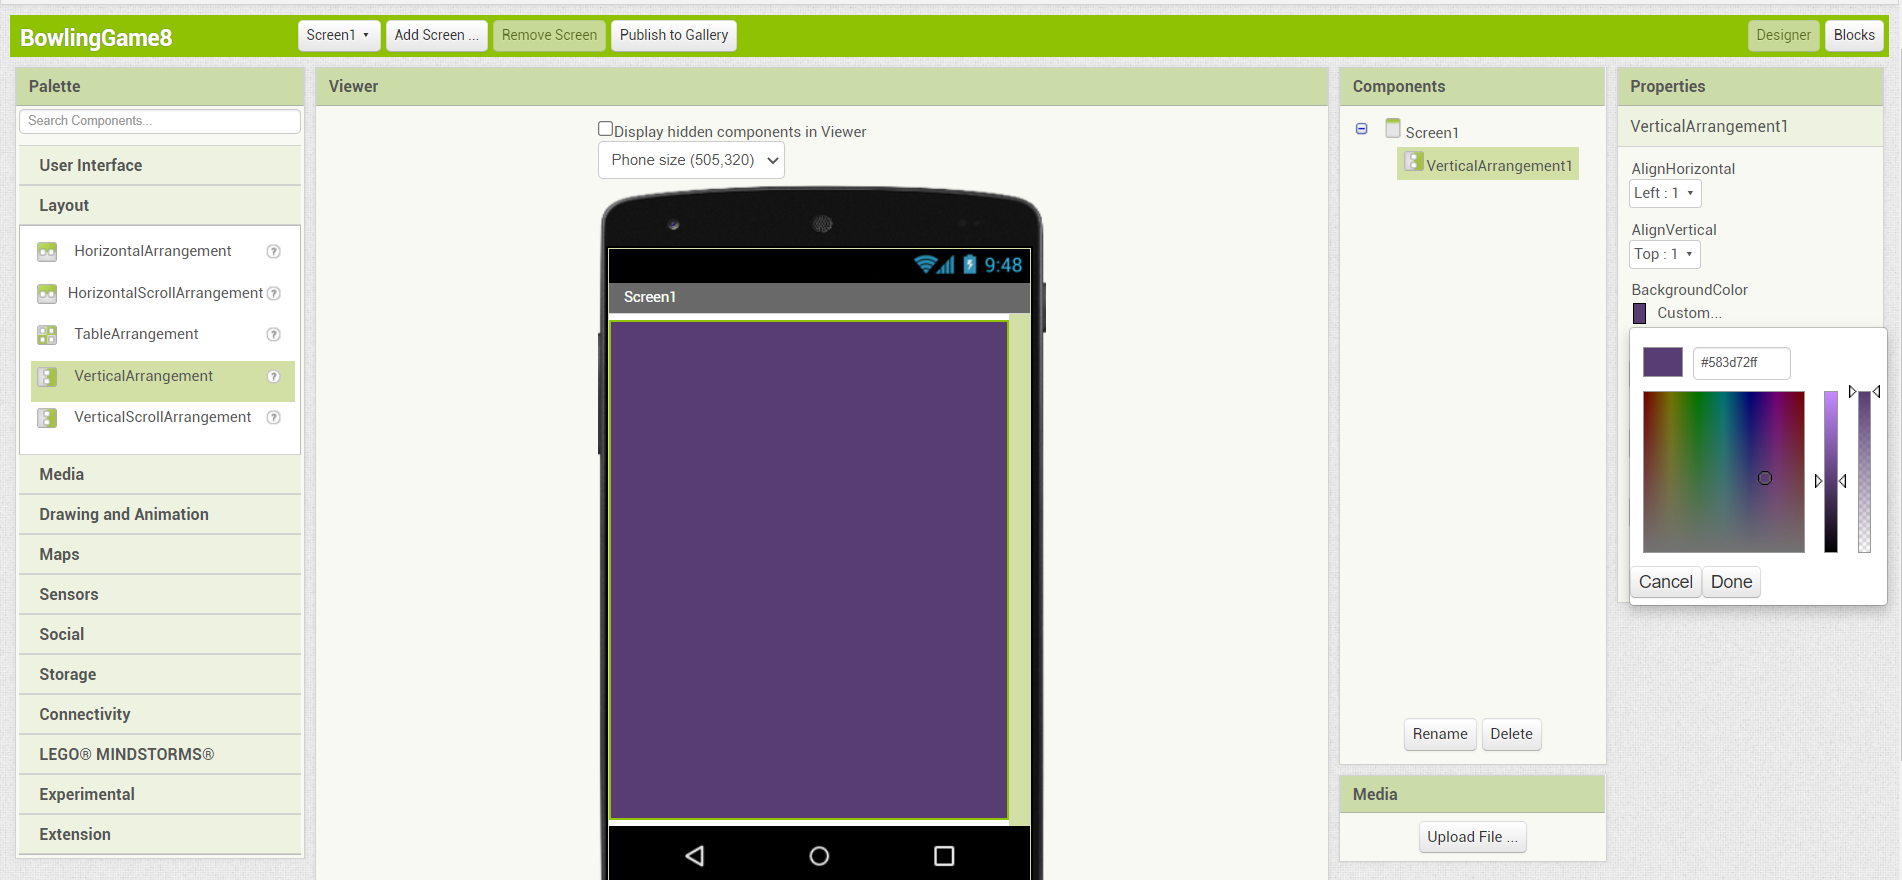
\includegraphics[width=1.0\linewidth,height=0.5\linewidth]{fig130002.png}
  \caption{Начален екран}
\label{fig130002}
\end{figure}

\section{Създаване на програмата}